% =============================================================================
%  ML pipeline overview (illustrative multi-panel figure)
%  pdflatex ml_pipeline.tex
%  Plots in zones 6 and 7 are schematic (no data); replace with your real plots if wanted.
% =============================================================================
\documentclass[tikz,border=6pt]{standalone}
\usepackage[T1]{fontenc}
\usepackage{helvet}
\renewcommand{\familydefault}{\sfdefault}
\usepackage{xcolor}
\usepackage{pifont}
\hyphenpenalty=10000 \exhyphenpenalty=10000
\usetikzlibrary{arrows.meta,calc,patterns,backgrounds}

% ---------------------------------------------------------------- palette
\definecolor{ink}{RGB}{44,52,62}
\definecolor{mblue}{RGB}{74,120,168}      % database-derived features
\definecolor{mgold}{RGB}{228,170,40}      % literature-derived features
\definecolor{mgrey}{RGB}{110,118,128}
\definecolor{zdb}{RGB}{250,230,235}   \definecolor{tdb}{RGB}{176,70,100}
\definecolor{zA}{RGB}{252,238,216}    \definecolor{tA}{RGB}{168,104,36}
\definecolor{zB}{RGB}{225,244,228}    \definecolor{tB}{RGB}{48,128,80}
\definecolor{zC}{RGB}{238,239,241}    \definecolor{tC}{RGB}{96,104,116}
\definecolor{zD}{RGB}{236,231,248}    \definecolor{tD}{RGB}{108,78,170}
\definecolor{zE}{RGB}{222,236,250}    \definecolor{tE}{RGB}{46,100,168}
\definecolor{zF}{RGB}{252,232,214}    \definecolor{tF}{RGB}{196,96,28}
\definecolor{leak}{RGB}{200,50,50}    \definecolor{okgreen}{RGB}{36,128,62}
% paper colours (Tableau-like, no red)
\definecolor{p1}{RGB}{76,120,168} \definecolor{p2}{RGB}{245,133,24} \definecolor{p3}{RGB}{84,162,75}
\definecolor{p4}{RGB}{178,121,162}\definecolor{p5}{RGB}{114,183,178}\definecolor{p6}{RGB}{238,202,59}
\definecolor{p7}{RGB}{157,117,93} \definecolor{p8}{RGB}{186,176,172}

\tikzset{
  flow/.style={-{Latex[length=1.8mm,width=1.4mm]},line width=0.7pt,draw=ink},
  bus/.style={line width=0.7pt,draw=ink},
  tflow/.style={-{Latex[length=2.6mm,width=2.2mm]},line width=1.7pt,draw=black!85},
  pcap/.style={font=\sffamily\fontsize{5.8}{6.7}\selectfont,text=black!62,align=center,inner sep=1pt},
  plab/.style={font=\sffamily\fontsize{6.2}{7.2}\selectfont,text=ink,inner sep=1pt},
  pmono/.style={font=\ttfamily\fontsize{5}{6.3}\selectfont,text=ink,anchor=west,inner sep=0pt},
  chip/.style={draw=ink,line width=0.4pt,rounded corners=1.5pt,inner sep=1.5pt,align=center,
    font=\sffamily\fontsize{5.8}{6.6}\selectfont,text=ink},
}
\newcommand{\pfzone}[6]{\draw[fill=#5,draw=#6,rounded corners=5pt,line width=0.6pt] (#1,#2) rectangle (#3,#4);}
\newcommand{\pftitle}[5]{%
  \node[circle,fill=#5,text=white,inner sep=0pt,minimum size=0.36cm,font=\sffamily\bfseries\fontsize{7}{8}\selectfont] at (#1,#2) {#3};
  \node[anchor=west,text=#5,font=\sffamily\bfseries\fontsize{7.6}{9}\selectfont,inner sep=0pt] at ({#1+0.26},{#2}) {#4};}
% feature matrix: top-left (x,y), cols, rows, cell w, cell h, colour, seed
\newcommand{\pfmat}[8]{%
  \pgfmathtruncatemacro{\pfC}{#3-1}\pgfmathtruncatemacro{\pfR}{#4-1}%
  \foreach \c in {0,...,\pfC}{\foreach \r in {0,...,\pfR}{%
    \pgfmathtruncatemacro{\k}{mod(\c*5+\r*3+#8,4)}\pgfmathsetmacro{\t}{24+18*\k}%
    \fill[#7!\t,draw=white,line width=0.3pt] ({#1+\c*#5},{#2-\r*#6}) rectangle ({#1+(\c+1)*#5},{#2-(\r+1)*#6});}}}
\newcommand{\pfdoi}[4]{\fill[mgrey,draw=white,line width=0.3pt] (#1,#2) rectangle ({#1+#3},{#2-#4});}
\newcommand{\pftarget}[4]{\draw[fill=white,draw=black!70,line width=0.4pt] (#1,#2) rectangle ({#1+#3},{#2-#4});
  \fill[pattern=north east lines,pattern color=black!60] (#1,#2) rectangle ({#1+#3},{#2-#4});
  \draw[black!70,line width=0.4pt] (#1,#2) rectangle ({#1+#3},{#2-#4});}
\newcommand{\pfpage}[5]{% x,y (bottom-left), w, h, fill
  \draw[fill=#5,draw=ink,line width=0.45pt] (#1,#2) -- ({#1+#3},#2) -- ({#1+#3},{#2+#4-0.2}) -- ({#1+#3-0.2},{#2+#4}) -- (#1,{#2+#4}) -- cycle;
  \draw[fill=white,draw=ink,line width=0.35pt] ({#1+#3-0.2},{#2+#4}) -- ({#1+#3-0.2},{#2+#4-0.2}) -- ({#1+#3},{#2+#4-0.2}) -- cycle;}
\newcommand{\pftree}[2]{% root position
  \draw[line width=0.5pt,draw=ink]
    (#1,#2) -- ({#1-0.26},{#2-0.34}) (#1,#2) -- ({#1+0.26},{#2-0.34})
    ({#1-0.26},{#2-0.34}) -- ({#1-0.4},{#2-0.68}) ({#1-0.26},{#2-0.34}) -- ({#1-0.12},{#2-0.68})
    ({#1+0.26},{#2-0.34}) -- ({#1+0.12},{#2-0.68}) ({#1+0.26},{#2-0.34}) -- ({#1+0.4},{#2-0.68});
  \fill[ink] (#1,#2) circle (0.075);
  \foreach \dx in {-0.26,0.26}{\fill[mgrey] ({#1+\dx},{#2-0.34}) circle (0.065);}
  \foreach \dx in {-0.4,-0.12,0.12,0.4}{\fill[okgreen!75] ({#1+\dx},{#2-0.68}) circle (0.055);}}
% 3x3 bin of paper-coloured devices: lower-left (x,y), colours (9 numbers as list), outline colour
\newcommand{\pfbin}[4]{% x, y, list, outline
  \draw[fill=white,draw=#4,line width=0.8pt,rounded corners=2pt] (#1,#2) rectangle ({#1+1.25},{#2+1.1});
  \pgfmathtruncatemacro{\pfidx}{0}
  \foreach \p [count=\n from 0] in {#3}{%
    \pgfmathtruncatemacro{\cc}{mod(\n,3)}\pgfmathtruncatemacro{\rr}{int(\n/3)}%
    \fill[p\p,draw=white,line width=0.3pt] ({#1+0.155+\cc*0.31},{#2+0.8-\rr*0.31}) rectangle ({#1+0.155+\cc*0.31+0.28},{#2+0.8-\rr*0.31+0.28});}}

\begin{document}
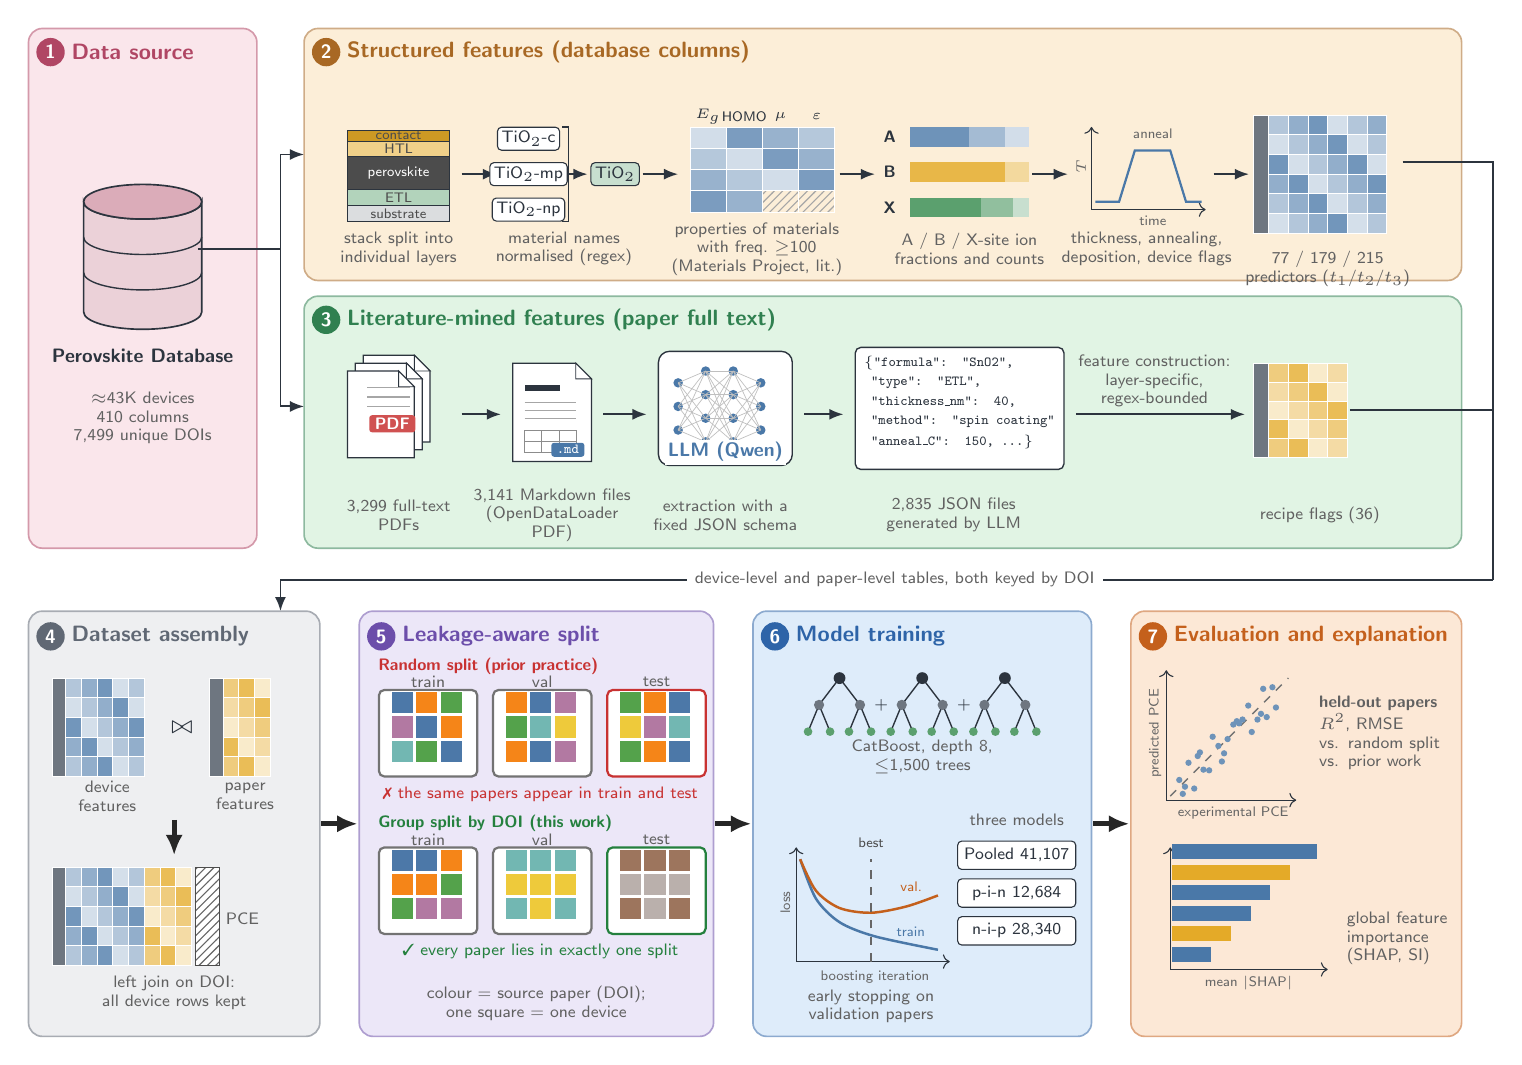
\begin{tikzpicture}[x=1cm,y=1cm]

% ====================================================================== ROW 1
\pfzone{0}{6.2}{2.9}{12.8}{zdb}{tdb!55}
\pfzone{3.5}{9.6}{18.2}{12.8}{zA}{tA!55}
\pfzone{3.5}{6.2}{18.2}{9.4}{zB}{tB!55}
\pftitle{0.28}{12.5}{1}{Data source}{tdb}
\pftitle{3.78}{12.5}{2}{Structured features (database columns)}{tA}
\pftitle{3.78}{9.1}{3}{Literature-mined features (paper full text)}{tB}

% ---- database cylinder
\begin{scope}[shift={(1.45,10.0)}]
  \draw[fill=tdb!25,draw=ink,line width=0.6pt] (-0.75,-0.8) arc (180:360:0.75 and 0.22) -- (0.75,0.6) arc (0:-180:0.75 and 0.22) -- cycle;
  \draw[line width=0.5pt,ink] (-0.75,-0.3) arc (180:360:0.75 and 0.22);
  \draw[line width=0.5pt,ink] (-0.75,0.15) arc (180:360:0.75 and 0.22);
  \draw[fill=tdb!45,draw=ink,line width=0.6pt] (0,0.6) ellipse (0.75 and 0.22);
\end{scope}
\node[plab,font=\sffamily\bfseries\fontsize{7.2}{8.4}\selectfont] at (1.45,8.65) {Perovskite Database};
\node[pcap,text width=2.6cm] at (1.45,7.85) {$\approx$43K devices\\410 columns\\7,499 unique DOIs};
% branches
\draw[bus] (2.15,10.0) -- (3.2,10.0);
\draw[bus] (3.2,11.2) -- (3.2,8.0);
\draw[flow] (3.2,11.2) -- (3.5,11.2);
\draw[flow] (3.2,8.0) -- (3.5,8.0);

% ---------------------------------------------------------------- lane A items
% A1 device stack
\begin{scope}[shift={(4.05,10.35)}]
  \draw[fill=mgrey!25,draw=ink,line width=0.4pt] (0,0) rectangle (1.3,0.2);
  \draw[fill=okgreen!35,draw=ink,line width=0.4pt] (0,0.2) rectangle (1.3,0.4);
  \draw[fill=black!70,draw=ink,line width=0.4pt] (0,0.4) rectangle (1.3,0.82);
  \draw[fill=mgold!55,draw=ink,line width=0.4pt] (0,0.82) rectangle (1.3,1.02);
  \draw[fill=mgold!90!black,draw=ink,line width=0.4pt] (0,1.02) rectangle (1.3,1.16);
  \node[font=\sffamily\fontsize{4.6}{5}\selectfont,text=white] at (0.65,0.61) {perovskite};
  \foreach \y/\t in {0.1/substrate,0.3/ETL,0.92/HTL,1.09/contact}{\node[font=\sffamily\fontsize{4.4}{5}\selectfont,text=black!70] at (0.65,\y) {\t};}
\end{scope}
\node[pcap,text width=1.9cm] at (4.7,10.0) {stack split into\\individual layers};
\draw[flow] (5.5,10.95) -- (5.95,10.95);
% A2 name normalisation
\node[chip,fill=white] (n1) at (6.35,11.4) {TiO$_2$-c};
\node[chip,fill=white] (n2) at (6.35,10.95) {TiO$_2$-mp};
\node[chip,fill=white] (n3) at (6.35,10.5) {TiO$_2$-np};
\draw[line width=0.5pt,ink] (6.78,11.55) -- (6.86,11.55) -- (6.86,10.35) -- (6.78,10.35);
\draw[flow] (6.86,10.95) -- (7.1,10.95);
\node[chip,fill=okgreen!25] at (7.45,10.95) {TiO$_2$};
\node[pcap,text width=1.9cm] at (6.8,10.0) {material names\\normalised (regex)};
\draw[flow] (7.8,10.95) -- (8.25,10.95);
% A3 property table
\foreach \c in {0,...,3}{\foreach \r in {0,...,3}{%
  \pgfmathtruncatemacro{\k}{mod(\c*3+\r*5,4)}
  \ifnum\r=3\ifnum\c>1
     \fill[pattern=north east lines,pattern color=black!35,draw=white,line width=0.3pt] ({8.4+\c*0.46},{11.55-\r*0.27}) rectangle ({8.4+(\c+1)*0.46},{11.55-(\r+1)*0.27});
  \else\fill[mblue!\the\numexpr25+16*\k\relax,draw=white,line width=0.3pt] ({8.4+\c*0.46},{11.55-\r*0.27}) rectangle ({8.4+(\c+1)*0.46},{11.55-(\r+1)*0.27});\fi
  \else\fill[mblue!\the\numexpr25+16*\k\relax,draw=white,line width=0.3pt] ({8.4+\c*0.46},{11.55-\r*0.27}) rectangle ({8.4+(\c+1)*0.46},{11.55-(\r+1)*0.27});\fi}}
\foreach \c/\t in {0/{$E_g$},1/{HOMO},2/{$\mu$},3/{$\varepsilon$}}{\node[font=\sffamily\fontsize{4.4}{5}\selectfont,text=ink] at ({8.4+\c*0.46+0.23},11.68) {\t};}
\node[pcap,text width=2.5cm] at (9.25,10.0) {properties of materials\\with freq.\ $\geq$100\\(Materials Project, lit.)};
\draw[flow] (10.3,10.95) -- (10.75,10.95);
% A4 ion fractions
\foreach \y/\s in {11.45/{p1/0.8/p2/0.6/p3/0.4},10.95/{p4/1.3/p5/0.5},10.45/{p6/0.9/p7/0.6/p8/0.3}}{}
\begin{scope}[shift={(11.2,0)}]
  \fill[mblue!80] (0,11.3) rectangle (0.75,11.55); \fill[mblue!50] (0.75,11.3) rectangle (1.2,11.55); \fill[mblue!25] (1.2,11.3) rectangle (1.5,11.55);
  \fill[mgold!85] (0,10.85) rectangle (1.2,11.1);   \fill[mgold!45] (1.2,10.85) rectangle (1.5,11.1);
  \fill[okgreen!75] (0,10.4) rectangle (0.9,10.65);  \fill[okgreen!50] (0.9,10.4) rectangle (1.3,10.65); \fill[okgreen!25] (1.3,10.4) rectangle (1.5,10.65);
  \foreach \y/\t in {11.425/A,10.975/B,10.525/X}{\node[font=\sffamily\bfseries\fontsize{5.6}{6}\selectfont,text=ink,anchor=east] at (-0.06,\y) {\t};}
\end{scope}
\node[pcap,text width=2.2cm] at (11.95,10.0) {A / B / X-site ion\\fractions and counts};
\draw[flow] (12.75,10.95) -- (13.2,10.95);
% A5 process
\begin{scope}[shift={(13.5,10.5)}]
  \draw[->,line width=0.4pt,ink] (0,0) -- (1.45,0); \draw[->,line width=0.4pt,ink] (0,0) -- (0,1.05);
  \draw[line width=0.8pt,mblue] (0.05,0.1) -- (0.35,0.1) -- (0.55,0.75) -- (1.0,0.75) -- (1.2,0.1) -- (1.4,0.1);
  \node[font=\sffamily\fontsize{4.6}{5}\selectfont,text=black!60] at (0.78,-0.14) {time};
  \node[font=\sffamily\fontsize{4.6}{5}\selectfont,text=black!60,rotate=90] at (-0.13,0.55) {$T$};
  \node[font=\sffamily\fontsize{4.6}{5}\selectfont,text=black!60,anchor=south] at (0.78,0.78) {anneal};
\end{scope}
\node[pcap,text width=2.2cm] at (14.2,10.0) {thickness, annealing,\\deposition, device flags};
\draw[flow] (15.05,10.95) -- (15.5,10.95);
% A6 output matrix
\pfdoi{15.55}{11.7}{0.2}{1.5}
\pfmat{15.75}{11.7}{6}{6}{0.25}{0.25}{mblue}{1}
\node[pcap,text width=2.4cm] at (16.5,9.75) {77 / 179 / 215\\predictors ($t_1$/$t_2$/$t_3$)};

% ---------------------------------------------------------------- lane B items
% B1 PDFs
\foreach \d in {0.2,0.1,0}{\pgfmathsetmacro{\px}{4.05+\d}\pgfmathsetmacro{\py}{7.35+\d}\pfpage{\px}{\py}{0.85}{1.1}{white}}
\node[fill=leak!85,text=white,font=\sffamily\bfseries\fontsize{5.6}{6}\selectfont,inner xsep=2pt,inner ysep=1pt,rounded corners=1pt] at (4.62,7.78) {PDF};
\foreach \y in {8.0,8.12,8.24}{\draw[black!35,line width=0.5pt] (4.3,\y) -- (4.85,\y);}
\node[pcap,text width=1.7cm] at (4.7,6.62) {3,299 full-text\\PDFs};
\draw[flow] (5.5,7.9) -- (6.0,7.9);
% B2 markdown
\pfpage{6.15}{7.3}{1.0}{1.25}{white}
\fill[ink] (6.3,8.2) rectangle (6.75,8.27);
\foreach \y in {8.05,7.95,7.85}{\draw[black!35,line width=0.5pt] (6.3,\y) -- (6.95,\y);}
\foreach \c in {0,1,2}{\foreach \r in {0,1}{\draw[black!45,line width=0.3pt] ({6.3+\c*0.22},{7.7-\r*0.14}) rectangle ({6.3+(\c+1)*0.22},{7.7-(\r+1)*0.14});}}
\node[fill=mblue,text=white,font=\ttfamily\fontsize{5}{5.6}\selectfont,inner xsep=2pt,inner ysep=1pt,rounded corners=1pt] at (6.85,7.45) {.md};
\node[pcap,text width=2.1cm] at (6.65,6.62) {3,141 Markdown files\\(OpenDataLoader PDF)};
\draw[flow] (7.3,7.9) -- (7.85,7.9);
% B3 LLM
\draw[fill=white,draw=ink,line width=0.5pt,rounded corners=4pt] (8.0,7.25) rectangle (9.7,8.7);
\foreach \x/\n in {8.25/3,8.6/4,8.95/4,9.3/3}{%
  \ifnum\n=3\foreach \y in {8.3,8.0,7.7}{\fill[mblue] (\x,\y) circle (0.06);}\else\foreach \y in {8.45,8.15,7.85,7.55}{\fill[mblue] (\x,\y) circle (0.06);}\fi}
\foreach \a in {8.3,8.0,7.7}{\foreach \b in {8.45,8.15,7.85,7.55}{\draw[black!25,line width=0.25pt] (8.25,\a) -- (8.6,\b); \draw[black!25,line width=0.25pt] (9.3,\a) -- (8.95,\b);}}
\foreach \a in {8.45,8.15,7.85,7.55}{\foreach \b in {8.45,8.15,7.85,7.55}{\draw[black!25,line width=0.25pt] (8.6,\a) -- (8.95,\b);}}
\node[font=\sffamily\bfseries\fontsize{6.6}{7.4}\selectfont,text=mblue,fill=white,inner sep=1pt] at (8.85,7.42) {LLM (Qwen)};
\node[pcap,text width=2.0cm] at (8.85,6.62) {extraction with a\\fixed JSON schema};
\draw[flow] (9.85,7.9) -- (10.35,7.9);
% B4 JSON
\draw[fill=white,draw=ink,line width=0.5pt,rounded corners=2pt] (10.5,7.2) rectangle (13.15,8.75);
\node[pmono] at (10.6,8.55) {\{"formula": "SnO2",};
\node[pmono] at (10.6,8.30) {\ "type": "ETL",};
\node[pmono] at (10.6,8.05) {\ "thickness\_nm": 40,};
\node[pmono] at (10.6,7.80) {\ "method": "spin coating"};
\node[pmono] at (10.6,7.55) {\ "anneal\_C": 150, ...\}};
\node[pcap,text width=2.5cm] at (11.75,6.62) {2,835 JSON files\\generated by LLM};
\draw[flow] (13.3,7.9) -- (15.45,7.9);
\node[pcap,text width=2.2cm,above] at (14.3,7.95) {feature construction:\\layer-specific, regex-bounded};
% B6 output matrix
\pfdoi{15.55}{8.55}{0.2}{1.2}
\pfmat{15.75}{8.55}{4}{5}{0.25}{0.24}{mgold}{2}
\node[pcap,text width=2.4cm] at (16.4,6.62) {recipe flags (36)};

% ---------------------------------------------------------------- merge connector
\draw[bus] (17.45,11.1) -- (18.6,11.1) -- (18.6,5.8);
\draw[bus] (16.78,7.95) -- (17.45,7.95); \draw[bus] (17.45,7.95) -- (18.6,7.95);
\draw[bus] (18.6,5.8) -- (3.2,5.8);
\draw[flow] (3.2,5.8) -- (3.2,5.4);
\node[pcap,fill=white,inner xsep=3pt] at (11.0,5.8) {device-level and paper-level tables, both keyed by DOI};

% ====================================================================== ROW 2
\pfzone{0}{0}{3.7}{5.4}{zC}{tC!55}
\pfzone{4.2}{0}{8.7}{5.4}{zD}{tD!55}
\pfzone{9.2}{0}{13.5}{5.4}{zE}{tE!55}
\pfzone{14.0}{0}{18.2}{5.4}{zF}{tF!55}
\draw[tflow] (3.72,2.7) -- (4.18,2.7);
\draw[tflow] (8.72,2.7) -- (9.18,2.7);
\draw[tflow] (13.52,2.7) -- (13.98,2.7);

% ---------------------------------------------------------------- 4 dataset assembly
\pftitle{0.28}{5.08}{4}{Dataset assembly}{tC}
\pfdoi{0.3}{4.55}{0.17}{1.25}
\pfmat{0.47}{4.55}{5}{5}{0.2}{0.25}{mblue}{1}
\node[font=\sffamily\bfseries\fontsize{9}{10}\selectfont,text=ink] at (1.95,3.92) {$\bowtie$};
\pfdoi{2.3}{4.55}{0.17}{1.25}
\pfmat{2.47}{4.55}{3}{5}{0.2}{0.25}{mgold}{2}
\node[pcap,text width=1.5cm] at (1.0,3.05) {device\\features};
\node[pcap,text width=1.5cm] at (2.75,3.05) {paper\\features};
\draw[tflow] (1.85,2.75) -- (1.85,2.3);
\pfdoi{0.3}{2.15}{0.17}{1.25}
\pfmat{0.47}{2.15}{5}{5}{0.2}{0.25}{mblue}{1}
\pfmat{1.47}{2.15}{3}{5}{0.2}{0.25}{mgold}{2}
\pftarget{2.12}{2.15}{0.3}{1.25}
\node[pcap,anchor=west,inner xsep=0pt] at (2.5,1.5) {PCE};
\node[pcap,text width=3.3cm] at (1.85,0.55) {left join on DOI:\\all device rows kept};

% ---------------------------------------------------------------- 5 leakage-aware split
\pftitle{4.48}{5.08}{5}{Leakage-aware split}{tD}
\node[plab,anchor=west,text=leak,font=\sffamily\bfseries\fontsize{6.2}{7}\selectfont] at (4.4,4.7) {Random split (prior practice)};
\foreach \x/\t in {4.45/train,5.9/val,7.35/test}{\node[pcap] at ({\x+0.625},4.5) {\t};}
\pfbin{4.45}{3.3}{1,2,3,4,1,2,5,3,1}{black!55}
\pfbin{5.9}{3.3}{2,1,4,3,5,6,2,1,4}{black!55}
\pfbin{7.35}{3.3}{3,2,1,6,4,5,3,2,1}{leak}
\node[pcap,text=leak,text width=4.2cm] at (6.5,3.08) {\textbf{\ding{55}} the same papers appear in train and test};
\node[plab,anchor=west,text=okgreen,font=\sffamily\bfseries\fontsize{6.2}{7}\selectfont] at (4.4,2.7) {Group split by DOI (this work)};
\foreach \x/\t in {4.45/train,5.9/val,7.35/test}{\node[pcap] at ({\x+0.625},2.5) {\t};}
\pfbin{4.45}{1.3}{1,1,2,2,2,3,3,4,4}{black!55}
\pfbin{5.9}{1.3}{5,5,5,6,6,6,5,6,5}{black!55}
\pfbin{7.35}{1.3}{7,7,7,8,8,8,7,8,7}{okgreen}
\node[pcap,text=okgreen,text width=4.2cm] at (6.5,1.08) {\textbf{\ding{51}} every paper lies in exactly one split};
\node[pcap,text width=4.2cm] at (6.45,0.42) {colour = source paper (DOI); one square = one device};

% ---------------------------------------------------------------- 6 training
\pftitle{9.48}{5.08}{6}{Model training}{tE}
\foreach \x in {10.3,11.35,12.4}{\pftree{\x}{4.55}}
\node[plab] at (10.83,4.2) {+}; \node[plab] at (11.88,4.2) {+};
\node[pcap,text width=4.0cm] at (11.35,3.55) {CatBoost, depth 8,\\$\leq$1,500 trees};
% early stopping plot
\begin{scope}[shift={(9.75,0.95)}]
  \draw[->,line width=0.4pt,ink] (0,0) -- (1.95,0); \draw[->,line width=0.4pt,ink] (0,0) -- (0,1.45);
  \draw[line width=0.9pt,mblue] plot[smooth] coordinates {(0.05,1.3) (0.25,0.8) (0.55,0.5) (1.0,0.32) (1.8,0.15)};
  \draw[line width=0.9pt,tF] plot[smooth] coordinates {(0.05,1.3) (0.25,0.9) (0.55,0.68) (0.95,0.62) (1.4,0.7) (1.8,0.84)};
  \draw[dashed,line width=0.5pt,black!60] (0.95,0) -- (0.95,1.3);
  \node[font=\sffamily\fontsize{4.8}{5.4}\selectfont,text=black!70,anchor=south] at (0.95,1.32) {best};
  \node[font=\sffamily\fontsize{4.8}{5.4}\selectfont,text=mblue,anchor=west] at (1.15,0.38) {train};
  \node[font=\sffamily\fontsize{4.8}{5.4}\selectfont,text=tF,anchor=west] at (1.2,0.95) {val.};
  \node[font=\sffamily\fontsize{4.8}{5.4}\selectfont,text=black!60] at (1.0,-0.2) {boosting iteration};
  \node[font=\sffamily\fontsize{4.8}{5.4}\selectfont,text=black!60,rotate=90] at (-0.14,0.75) {loss};
\end{scope}
\node[pcap,text width=2.2cm] at (10.7,0.38) {early stopping on\\validation papers};
% three models
\node[pcap,text width=1.6cm] at (12.55,2.75) {three models};
\foreach \y/\t in {2.3/{Pooled 41,107},1.82/{p-i-n 12,684},1.34/{n-i-p 28,340}}{
  \node[chip,fill=white,minimum width=1.5cm,minimum height=0.36cm] at (12.55,\y) {\t};}

% ---------------------------------------------------------------- 7 evaluation
\pftitle{14.28}{5.08}{7}{Evaluation and explanation}{tF}
\begin{scope}[shift={(14.45,3.0)}]
  \draw[->,line width=0.4pt,ink] (0,0) -- (1.65,0); \draw[->,line width=0.4pt,ink] (0,0) -- (0,1.65);
  \draw[dashed,line width=0.5pt,black!55] (0.05,0.05) -- (1.55,1.55);
  \foreach \i in {1,...,26}{%
    \pgfmathsetmacro{\xx}{0.12+1.3*mod(\i*0.618034,1)}
    \pgfmathsetmacro{\yy}{max(0.08,min(1.55,\xx+0.22*sin(mod(\i*\i*13.7,360))))}
    \fill[mblue!80] (\xx,\yy) circle (0.04);}
  \node[font=\sffamily\fontsize{4.8}{5.4}\selectfont,text=black!60] at (0.85,-0.16) {experimental PCE};
  \node[font=\sffamily\fontsize{4.8}{5.4}\selectfont,text=black!60,rotate=90] at (-0.14,0.85) {predicted PCE};
\end{scope}
\node[pcap,anchor=west,text width=1.7cm,align=left] at (16.35,3.85) {\textbf{held-out papers}\\$R^2$, RMSE\\vs. random split\\vs. prior work};
\begin{scope}[shift={(14.5,0.85)}]
  \draw[->,line width=0.4pt,ink] (0,0) -- (0,1.55); \draw[->,line width=0.4pt,ink] (0,0) -- (2.0,0);
  \foreach \y/\w/\c in {1.4/1.85/mblue,1.14/1.5/mgold,0.88/1.25/mblue,0.62/1.0/mblue,0.36/0.75/mgold,0.1/0.5/mblue}{
    \fill[\c] (0.02,\y) rectangle ({0.02+\w},{\y+0.19});}
  \node[font=\sffamily\fontsize{4.8}{5.4}\selectfont,text=black!60] at (1.0,-0.17) {mean $|$SHAP$|$};
\end{scope}
\node[pcap,text width=1.5cm,anchor=north west,align=left] at (16.7,1.62) {global feature\\importance (SHAP, SI)};

\end{tikzpicture}
\end{document}